%!TEX root = ../report.tex

This chapter explores 3D geovisualisation techniques that could be applied to the project, discusses the World Wide Web as a platform for geovisualisations and common interactions found in 3D geovisualisations. Finally, the applications of geovisualisations are analysed and an overview of the project is provided from this research.

\section{3D geovisualisation techniques} {

	\textcite{bleisch2012geovisualization} defines two distinct categories that represent most 3D geovisualisations: 3D representations of the real world and a combination of 3D representations of the real world with abstract data.

	The \emph{3D representations of the real world} category represents the real world and its objects in realistic or generalised ways to communicate information. This category often uses x, y and z coordinates to show the real world dimensions \textendash\, easting, northing, elevation and sometimes the height of buildings or other objects. A 3D environment attempting to represent the real world usually consists of a digital elevation or surface model with either high resolution orthoimagery, satellite imagery or maps~\parencite{bleisch2012geovisualization}.

	\begin{figure}
	\centering
	\captionsetup{font=small}
    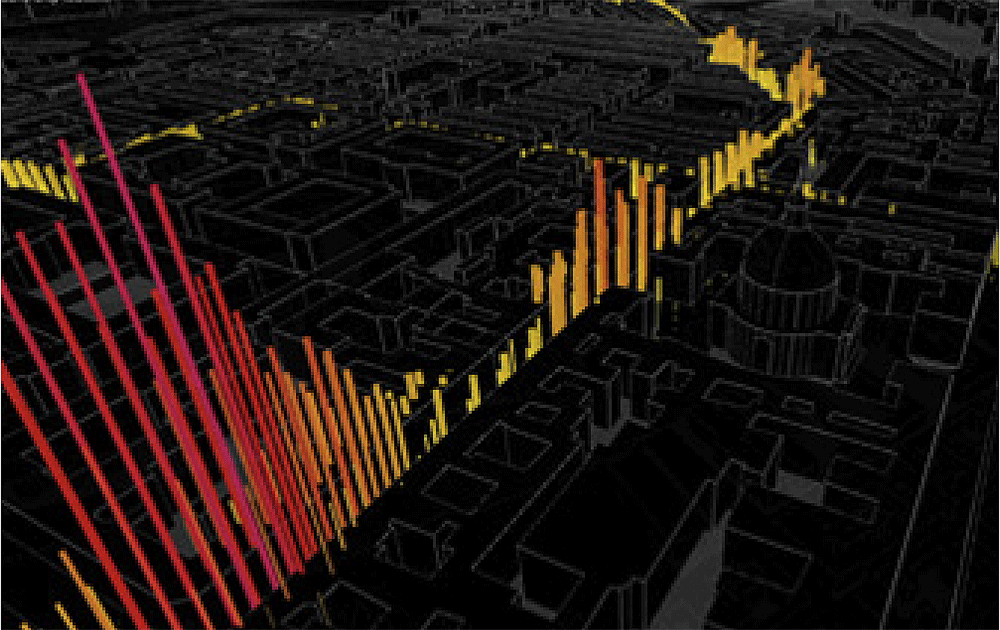
\includegraphics[width=0.8\textwidth]{images/literature/category-combination}
	\caption{An example of combining 3D representations of the real world with abstract data. \protect\footnotemark}
	\label{fig:category_combination}
\end{figure}

\footnotetext{\bibentry{ratti2010copenhagen}}


	Common examples of this category are digital city models and virtual globes. 3D city models often apply photo texturing to suggest additional detail, since the detail may not be present in the underlying geometric model of the city~\parencite{bleisch2012geovisualization}.

	In the \emph{combination of 3D representations of the real world with abstract data} category, the representation of the real world environment is enhanced with the inclusion of data displays. This category aims to communicate, analyse and explore data, where real world dimensions and data values are depicted through the x, y and z axes. An example of this category is shown in Figure~\ref{fig:category_combination} \parencite{bleisch2012geovisualization}.

	To visualise the data displays in this category, triangle based meshes, texture maps or non-uniform rational B-spline surfaces (NURBS) can be created and applied to the visualisation. NURBS in particular are computationally efficient and effective at modelling complex structures~\parencite{hildebrandt2011image, zhong2006enhanced}.

}

\section{Geovisualisations using the World Wide Web} {

	Geovisualisations can be realised through the World Wide Web, which has become a prominent medium for publishing geospatial data. The web facilitates the creation of immersive and highly interactive environments, which can be taken advantage of to explore and present dynamic geospatial data~\parencite{maceachren2001research}.

	WebGL is a cross-platform web standard for a 3D graphics API derived from OpenGL, which has been exposed through the HTML5 canvas element~\parencite{marrin2011webgl} as a drawing context. It is widely supported in modern browsers, without needing additional plug-ins or extensions, and is designed for building dynamic applications that require 3D visualisations~\parencite{chaturvedi2015web, marrin2011webgl, parisi2012webgl}. Rendering such visualisations in real-time is possible due to the accelerated graphics rendering provided by WebGL, which utilises the graphics card memory on a device~\parencite{chaturvedi2015web} to perform multiple operations in parallel to one another.

}

\section{Interaction in geovisualisations} {

	The communication between a user and a system, otherwise known as \emph{interaction}, is an important aspect in geovisualisation. Interaction enables users to explore the data presented to them in order to uncover trends and allow for decision-making processes~\parencite{yi2007toward}. It is also essential for visualisations to support interaction, otherwise the usefulness of the visualisation is greatly limited as the dataset that it represents grows larger~\parencite{yi2007toward}.

	In the context of geovisualisation, the user should be able to navigate the visualisation itself and the synthetic geography that it represents. Navigation enables particular and pertinent information to be located more successfully and is considered to be one of the most important metaphors for dynamic cartography~\parencite{cartwright2001geospatial}. The navigation of a geospatial representation requires the user to perform standard operations, which include: translate, scale, rotate, map projection, manipulation of the design representation parameters, level of generalisation and field of view~\parencite{cartwright2001geospatial, hand1997survey}.

}

\section{Applications of geovisualisation} {

	% equipped assist

	There is a comprehensive amount of geospatial data available, which has been made accessible through various digital data resources. Census enumerations, health statistics, land use categories, meteorological measurements, telephone information and transportation records constitute examples of geospatially referenced data that can be applied to geovisualisations for scientific, research and societal purposes. Furthermore, this widely accessible geospatial data has resulted in an equally large range of application domains for geovisualisations, which include earth science, public health and social science as shown in Figure~\ref{fig:geovisualisation_applications} \parencite{maceachren2004geovisualization}.

	\newcommand{\applicationwidth}{0.32\textwidth}
\newcommand{\applicationheight}{3cm}
\begin{figure}[H]
	\centering
    \begin{subfigure}[b]{\applicationwidth}
        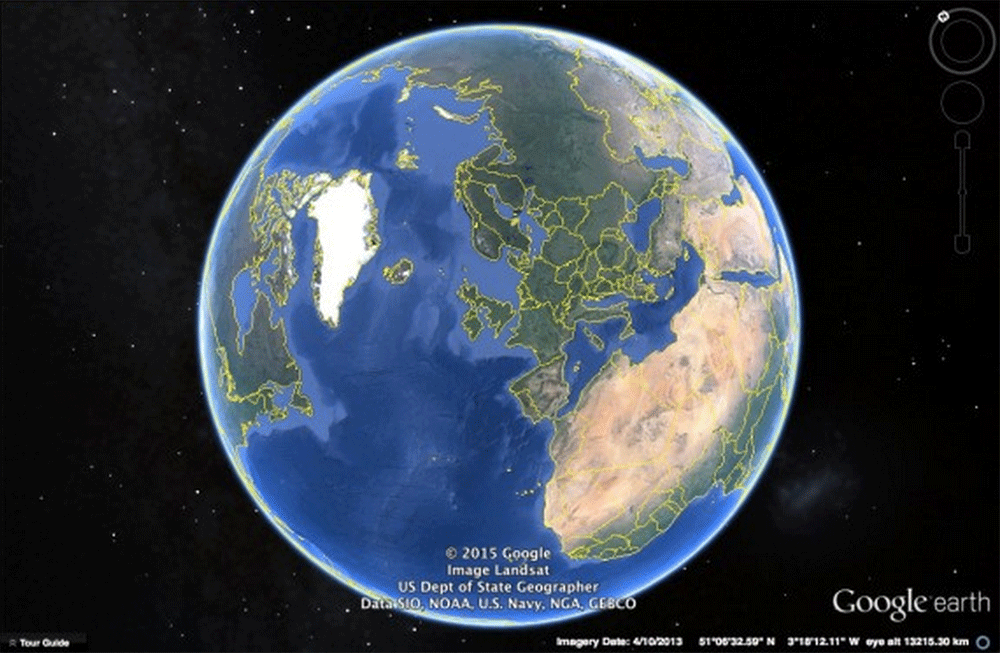
\includegraphics[width=\textwidth,height=\applicationheight]{images/literature/earth-science}
        \caption{Earth science \parencite{google2015earth}}
        % \protect\footnotemark}
        \label{fig:earth_science}
    \end{subfigure}
    \begin{subfigure}[b]{\applicationwidth}
        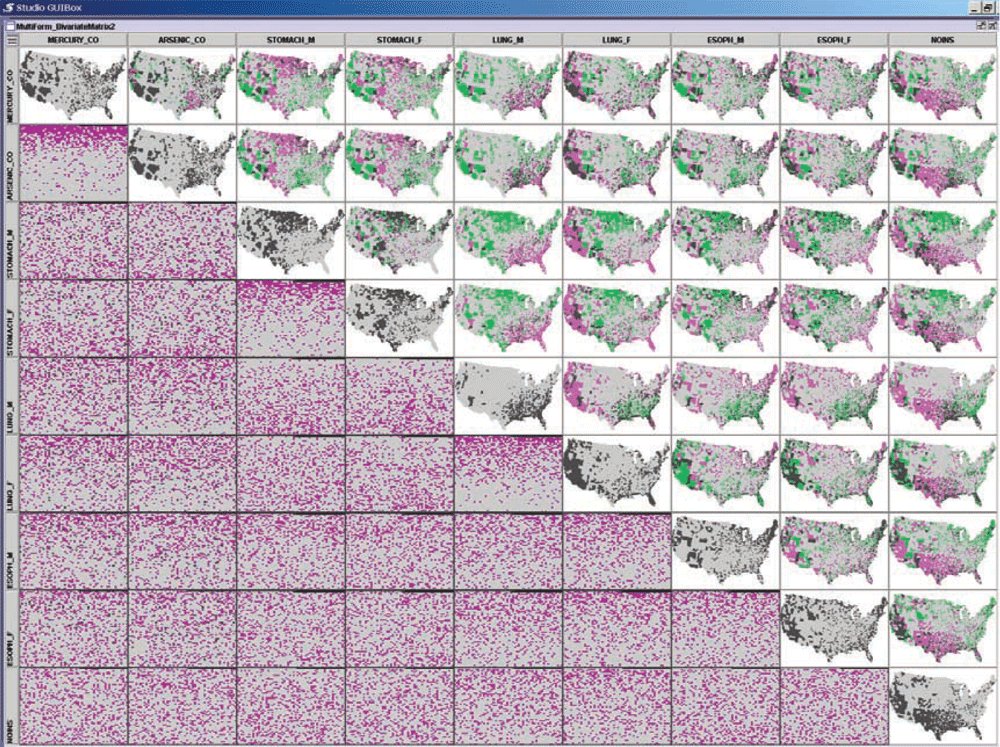
\includegraphics[width=\textwidth,height=\applicationheight]{images/literature/public-health}
        	\caption{\tiny{Public health \parencite{maceachren2004geovisualization}}}
        \label{fig:public_health}
    \end{subfigure}
    \begin{subfigure}[b]{\applicationwidth}
        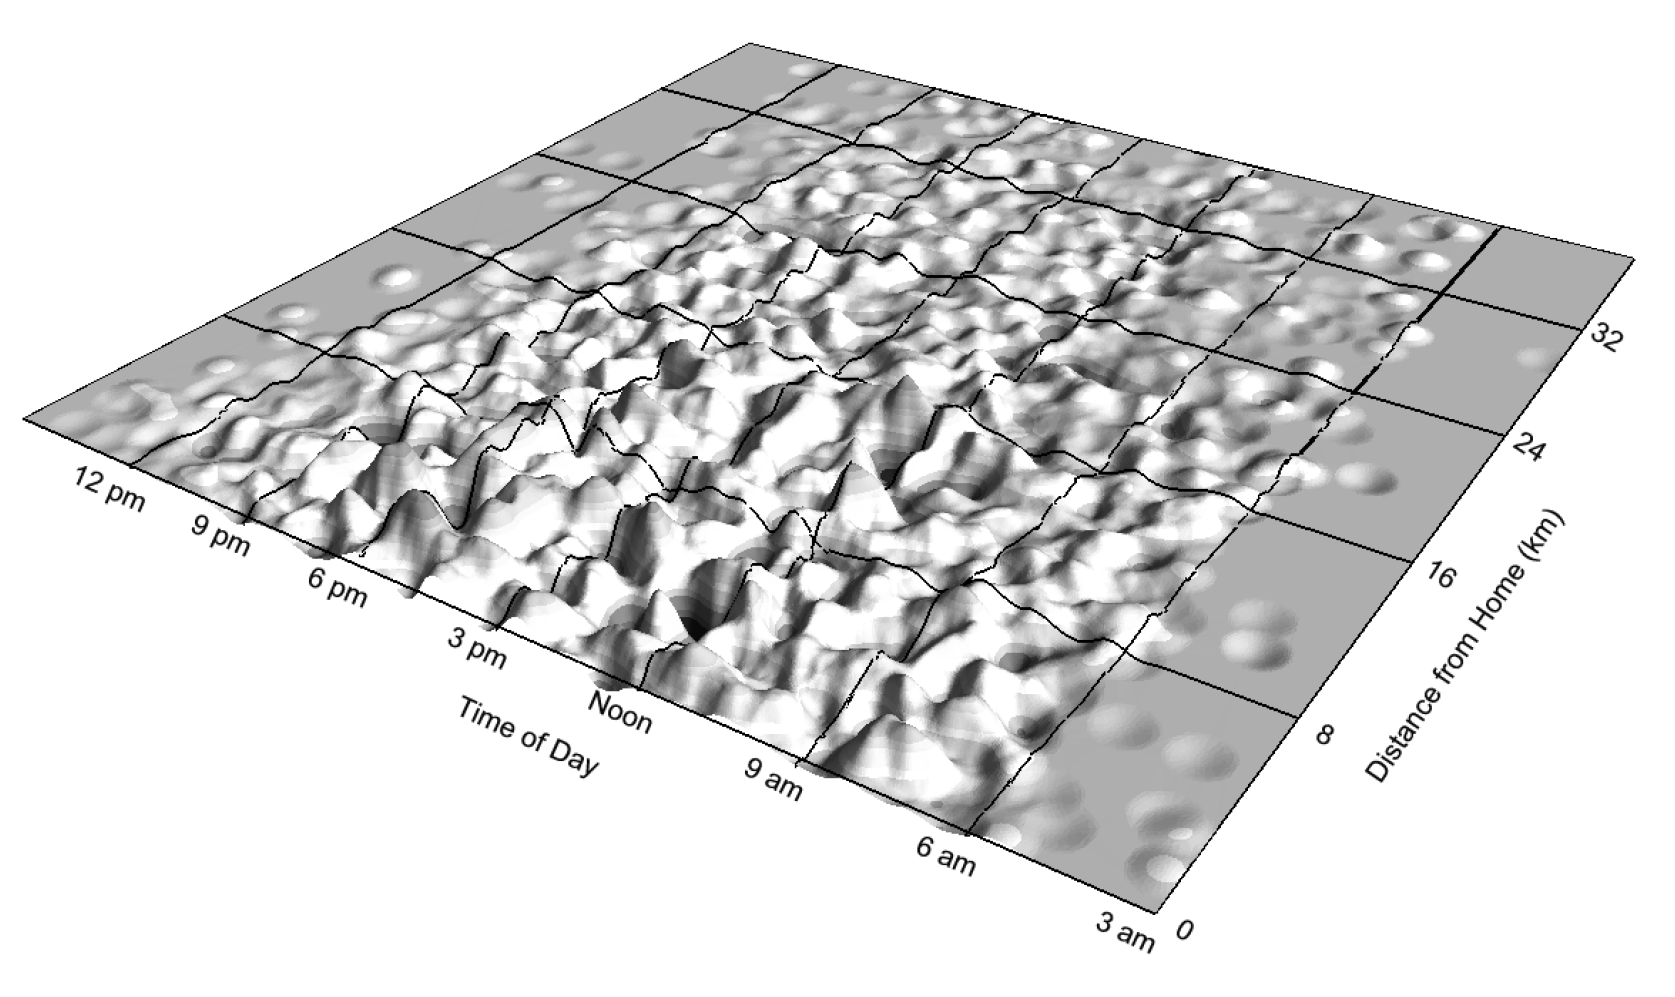
\includegraphics[width=\textwidth,height=\applicationheight]{images/literature/social-science}
        	\caption{Social science \parencite{kwan2004geovisualization}}
        \label{fig:social_science}
    \end{subfigure}
	\caption{Examples of geovisualisations used in various application domains.}
	\subfigcaptionskip
	\label{fig:geovisualisation_applications}
\end{figure}

% \footnotetext{\bibentry{google2015earth}}

	% Earth science
	In the domain of \emph{earth science}, the visualisation of environmental data reveals new insights into the patterns of nature and human-related phenomena. These visualisations also help improve the understanding of the dynamic processes of earth systems~\parencite{yu2012google}.

	\textcite{yu2012google} analyses virtual globes as a tool in earth science applications, which have been developed to effectively facilitate data collection, exploration and the visualisation of environmental data. They deliver huge volumes of satellite imagery, 3D views of the earth, topographic maps and distance measurement to the general public. These globes have promoted entertainment, education, the exploration of new findings, data sharing and provided researchers with effective channels of communicating their findings. Virtual globes can be applied to many areas and in the case of \emph{Google Earth}, typically focus on large-scale phenomena in the atmosphere, carbon science, ecosystems, energy, geology and natural disasters.

	% Public health
	Within \emph{public health}, geovisualisations can be modelled to geospatial data concerning risk factors, health outcomes and interventions to provide an opportunity to understand and act on the varied geographic distribution of disease. However, these datasets are typically difficult to analyse through traditional methods as the data is highly multivariate~\parencite{maceachren2004geovisualization}.

	\textcite{maceachren2004geovisualization} were able to apply a mortality and risk factor dataset to a geovisualisation, in order to explore the spatial and nonspatial relationships in this data. They considered environmental risk factors, health care access and cancer mortality rates of various ages and genders to demonstrate that it is possible to utilise geovisualisations in a way that addresses critical issues in public health.

	% Social science
	An important research area in \emph{social science} is the study of human activities and movements in space and time. Geovisualisations can model this data, which has become feasible with the increased availability of georeferenced individual-level data~\parencite{kwan2004geovisualization}.

	\textcite{kwan2004geovisualization} studied gender and ethnic differences in space-time activity patterns in a metropolitan area. Their study demonstrated that geovisualisation methods are effective in revealing the complex interaction between the spatial and temporal dimensions in structuring human spatial behaviour. \citeauthor{kwan2004geovisualization} also discovered that geovisualisation tools can help formulate more realistic computational or behavioural models for exploratory spatial data analysis.

}

\section{Overview} {

	In this work, HTML5 and WebGL will be used to visualise geographical data, with triangle based meshes and NURBS surface data displays. This ensures the development of a cross-platform system capable of rendering complex visualisations through accelerated graphics rendering. This project will consider several navigation interaction techniques, particularly translation, scaling and rotation. Finally, the visualisations will be applied to both earth and social science datasets as both domains have a wide array of applications.

}
